\documentclass[
	12pt,
	BCOR=5mm,
	DIV=12,
	headinclude=on,
	footinclude=off,
	parskip=half,
	bibliography=totoc,
	listof=entryprefix,
	toc=listof,
	numbers=noenddot,
	plainfootsepline
]{scrreprt}

%	Konfigurationsdatei einziehen
% !TEX root =  master.tex

%		LANGUAGE SETTINGS AND FONT ENCODING 
%
\usepackage[ngerman]{babel} 	% German language
\usepackage[utf8]{inputenc}
\usepackage[german=quotes]{csquotes} 	% correct quotes using \enquote{}
\usepackage[T1]{fontenc}


%\usepackage[english]{babel}   % For english language
%\usepackage{csquotes} 	% Richtiges Setzen der Anführungszeichen mit \enquote{}

% 		HYPERREF
%
\usepackage[
	hidelinks=true % keine roten Markierungen bei Links
]{hyperref}

% Zwei eigene Befehle zum Setzen von Autor und Titel. Ausserdem werden die PDF-Informationen richtig gesetzt.
\newcommand{\TitelDerArbeit}[1]{\def\DerTitelDerArbeit{#1}\hypersetup{pdftitle={#1}}}
\newcommand{\AutorDerArbeit}[1]{\def\DerAutorDerArbeit{#1}\hypersetup{pdfauthor={#1}}}
\newcommand{\Firma}[1]{\def\DerNameDerFirma{#1}}
\newcommand{\Kurs}[1]{\def\DieKursbezeichnung{#1}}

\newcommand{\heading}[1]{\textbf{#1}}

% Correct superscripts 
\usepackage{fnpct}


% Tabellen
\usepackage{ltablex}
\newcolumntype{s}{>{\hsize=.75\hsize}X}

%		CALCULATIONS
%
\usepackage{calc} % Used for extra space below footsepline


%		BIBLIOGRAPHY SETTINGS
%

% Uncomment the next three lines for author-year-style with footnotes (Chicago)
\usepackage[backend=biber, autocite=footnote, style=authoryear, dashed=false]{biblatex} 	%Use Author-Year-Cites with footnotes
\AdaptNoteOpt\footcite\multfootcite   %will add  separators if footcite is called multiple consecutive times 
\AdaptNoteOpt\autocite\multautocite % will add  separators if autocite is called multiple consecutive times

% Uncomment the next line for IEEE-style 
% \usepackage[backend=biber, autocite=inline, style=ieee]{biblatex} 	% Use IEEE-Style (e.g. [1])

% Uncomment the next line for alphabetic style 
% \usepackage[backend=biber, autocite=inline, style=alphabetic]{biblatex} 	% Use alphabetic style (e.g. [TGK12])

% Uncomment the next two lines vor Harvard-Style 
%\usepackage[backend=biber, style=apa]{biblatex} 	
%\DeclareLanguageMapping{german}{german-apa}


\DefineBibliographyStrings{ngerman}{  %Change u.a. to et al. (german only!)
	andothers = {{et\,al\adddot}},
}

%%% Uncomment the following lines to support hard URL breaks in bibliography 
%\apptocmd{\UrlBreaks}{\do\f\do\m}{}{}
%\setcounter{biburllcpenalty}{9000}% Kleinbuchstaben
%\setcounter{biburlucpenalty}{9000}% Großbuchstaben


\setlength{\bibparsep}{\parskip}		%add some space between biblatex entries in the bibliography
\addbibresource{bibliography.bib}	%Add file bibliography.bib as biblatex resource


%		FOOTNOTES 
%
% Count footnotes over chapters
\usepackage{chngcntr}
\counterwithout{footnote}{chapter}

%	ACRONYMS
%%%
%%% WICHTIG: Installieren Sie das neueste Acronyms-Paket!!!
%%%
\makeatletter
\usepackage[printonlyused]{acronym}
\@ifpackagelater{acronym}{2015/03/20}
  {%
    \renewcommand*{\aclabelfont}[1]{\textbf{\textsf{\acsfont{#1}}}}
  }%
  {%
  }%
\makeatother

%		LISTINGS
\usepackage{listings}	%Format Listings properly
\usepackage{xcolor}
\renewcommand{\lstlistingname}{Quelltext} 
\renewcommand{\lstlistlistingname}{Quelltextverzeichnis}
\lstset{numbers=left,
	numberstyle=\tiny,
	captionpos=b,
  basicstyle=\ttfamily\small,
  tabsize=2
}
\colorlet{punct}{red!60!black}
\definecolor{delim}{RGB}{20,105,176}
\colorlet{numb}{magenta!60!black}
\lstdefinelanguage{json}{
    basicstyle=\normalfont\ttfamily,
    numbers=left,
    numberstyle=\scriptsize,
    stepnumber=1,
    numbersep=8pt,
    showstringspaces=false,
    breaklines=true,
    frame=lines,
    literate=
     *{0}{{{\color{numb}0}}}{1}
      {1}{{{\color{numb}1}}}{1}
      {2}{{{\color{numb}2}}}{1}
      {3}{{{\color{numb}3}}}{1}
      {4}{{{\color{numb}4}}}{1}
      {5}{{{\color{numb}5}}}{1}
      {6}{{{\color{numb}6}}}{1}
      {7}{{{\color{numb}7}}}{1}
      {8}{{{\color{numb}8}}}{1}
      {9}{{{\color{numb}9}}}{1}
      {:}{{{\color{punct}{:}}}}{1}
      {,}{{{\color{punct}{,}}}}{1}
      {\{}{{{\color{delim}{\{}}}}{1}
      {\}}{{{\color{delim}{\}}}}}{1}
      {[}{{{\color{delim}{[}}}}{1}
      {]}{{{\color{delim}{]}}}}{1},
}


%		EXTRA PACKAGES
\usepackage{lipsum}    %Blindtext
\usepackage{microtype} % für bessere Silbentrennung
\usepackage{graphicx} % use various graphics formats
\usepackage[german]{varioref} 	% nicer references \vref
\usepackage{caption}	%better Captions
\usepackage{booktabs} %nicer Tabs
\usepackage{array}
%\newcolumntype{P}[1]{>{\raggedright\arraybackslash}p{#1}}

%   MATH-SUFF
\usepackage{amsthm}
\usepackage{amsmath}
\usepackage{amssymb}
\theoremstyle{definition}
\newtheorem{definition}{Definition}[section]
\newtheorem{example}{Beispiel}[section]
\newtheorem{problem}{Problem}[section]


%		ALGORITHMS
% \usepackage{algorithm}
% \usepackage{algpseudocode}
% \renewcommand{\listalgorithmname}{Algorithmenverzeichnis }
% \floatname{algorithm}{Algorithmus}


%		FONT SELECTION: Entweder Latin Modern oder Times / Helvetica
\usepackage{lmodern} %Latin modern font
%\usepackage{mathptmx}  %Helvetica / Times New Roman fonts (2 lines)
%\usepackage[scaled=.92]{helvet} %Helvetica / Times New Roman fonts (2 lines)

%		PAGE HEADER / FOOTER
%	    Warning: There are some redefinitions throughout the master.tex-file!  DON'T CHANGE THESE REDEFINITIONS!
\usepackage[automark,headsepline,footsepline]{scrlayer-scrpage}
% \RequirePackage[automark,headsepline,footsepline]{scrpage2}
\pagestyle{scrheadings}
\renewcommand*{\pnumfont}{\upshape\sffamily}
\renewcommand*{\headfont}{\upshape\sffamily}
\renewcommand*{\footfont}{\upshape\sffamily}
\renewcommand{\chaptermarkformat}{}
\RedeclareSectionCommand[beforeskip=0pt]{chapter}
\clearscrheadfoot

\ifoot[\rule{0pt}{\ht\strutbox+\dp\strutbox}DHBW Mannheim]{\rule{0pt}{\ht\strutbox+\dp\strutbox}DHBW Mannheim}
\ofoot[\rule{0pt}{\ht\strutbox+\dp\strutbox}\pagemark]{\rule{0pt}{\ht\strutbox+\dp\strutbox}\pagemark}

\ohead{\headmark}


\begin{document}

\TitelDerArbeit{Entwurf und Implementierung einer Referenzarchitektur zur automatischen Erzeugung digitaler Zwillinge}
\AutorDerArbeit{Aaron Schweig}
\Firma{Hays AG}
\Kurs{WWI18SEC}

\begin{titlepage}
\begin{minipage}{\textwidth}
		\vspace{-2cm}
		\noindent 
		% \includegraphics[scale=0.71]{img/firmenlogo.jpg} 
		\hfill   
\includegraphics{img/logo.jpg}
\end{minipage}
\vspace{1em}
\sffamily
\begin{center}
	\textsf{\large{}Duale Hochschule Baden-W\"urttemberg\\[1.5mm] Mannheim}\\[2em]
	\textsf{\textbf{\Large{}Bachelorarbeit}}\\[3mm]
	\textsf{\textbf{\DerTitelDerArbeit}} \\[1.5cm]
	\textsf{\textbf{\Large{}Studiengang Wirtschaftsinformatik}\\[3mm] \textsf{Studienrichtung Software Engineering}}
	
	\vspace{3em}
	% \textsf{\Large{Sperrvermerk}}
\vfill

\begin{minipage}{\textwidth}

\begin{tabbing}
	Wissenschaftlicher Betreuer: \hspace{0.85cm}\=\kill
	Verfasser/in: \> \DerAutorDerArbeit \\[1.5mm]
	Matrikelnummer: \> 6161622 \\[1.5mm]
	Firma: \> \DerNameDerFirma  \\[1.5mm]
	Abteilung: \> Softwareentwicklung \\[1.5mm]
	Kurs: \> \DieKursbezeichnung \\[1.5mm]
	Studiengangsleiter: \> Prof. Dr. Sebastian Ritterbusch  \\[1.5mm]
	Wissenschaftlicher Betreuer: \> Prof. Dr. Julian Reichwald \\
	\> j.reichwald@hs-mannheim.de \\
	% \> +49 151 / 123 456 \\[1.5mm]
	Firmenbetreuer: \> Daniel Kissel \\
	\> daniel.kissel@hays.de \\
	% \> +49 151 / 123 456 \\[1.5mm]
	Bearbeitungszeitraum: \> 15.11.2020 -- 15.02.2021
\end{tabbing}
\end{minipage}

\end{center}

\end{titlepage}


% Ehrenwörtliche Erklärung ewerkl.tex einziehen
% !TEX root =  master.tex

\clearpage
\chapter*{Ehrenwörtliche Erklärung}

% Wird die folgende Zeile auskommentiert, erscheint die ehrenwörtliche
% Erklärung im Inhaltsverzeichnis.

% \addcontentsline{toc}{chapter}{Ehrenwörtliche Erklärung}
Ich versichere hiermit, dass ich die vorliegende Arbeit
 mit dem Thema: \textit{\DerTitelDerArbeit} selbstständig verfasst und keine anderen als die angegebenen Quellen und
Hilfsmittel benutzt habe. Ich versichere zudem,
dass die eingereichte elektronische Fassung mit der gedruckten Fassung übereinstimmt.

\vspace{3cm}
Mannheim, \today \hfill \DerAutorDerArbeit


\pagenumbering{roman} % Römische Seitennummerierung
\normalfont

%	Kurzfassung
\chapter*{Kurzfassung}
\begingroup
\begin{table}[h!]
\setlength\tabcolsep{0pt}
\begin{tabular}{p{3.7cm}p{11.7cm}}
Titel: & \DerTitelDerArbeit \\
Verfasser/in: & \DerAutorDerArbeit \\
Kurs: & \DieKursbezeichnung \\
Ausbildungsstätte: & \DerNameDerFirma\\
\end{tabular}
\end{table}
\endgroup

Folgende Arbeit beschreibt ein Konzept für eine graphbasierte Service-Registry. Dabei wurde eine Gegenüberstellung zwischen dem hergeleiteten Konzept der Service-Registry und einer Komposition verschiedener Produkte zur Lösung desselben Problems durchgeführt. Ein Ergebnis dieser Gegenüberstellung war, dass sich die unterschiedlichen Produkte sehr gut ergänzen können, da sie verschiedene Probleme lösen.\\ Zu Beginn der Arbeit wurde noch eine Defintion von Microservices auf Basis ihrer Eigenschaften vorgenommen. Des weiteren wurden wichtige Konzepte von Microservices, \textit{Observability} und \textit{Governance}, beschrieben, um eine klare Basis zu schaffen auf der Kriterien definiert wurden, die in dem Vergleich genutzt wurden. Außerdem wurde mithilfe von Grundlagen aus der Graphentheorie erläutert, wieso Graphen und im speziellen Flüsse eine passende Datenstruktur zur Darstellung von Abhängigkeiten zwischen Services sind. Dabei wurde sowohl eine Kapazitätsfunktion, als auch eine Flussfunktion zur mathematischen Repräsentation des Graphen definiert.




%	Inhaltsverzeichnis
\tableofcontents

%	Abbildungsverzeichnis
\listoffigures

%	Tabellenverzeichnis
% \listoftables

%	Listingverzeichnis
% \lstlistoflistings

% 	Abkürzungsverzeichnis (siehe Datei acronyms.tex!)
\clearpage
\chapter*{Abkürzungsverzeichnis}	
\addcontentsline{toc}{chapter}{Abkürzungsverzeichnis}


\begin{acronym}
	\acro{DHBW}{Duale Hochschule Baden-Württemberg}
	\acro{IoT}{Internet of Things}
	\acro{DT}{Digitaler Zwilling}
	\acro{PHM}{Prognostics \& Health Management}
	\acro{MQTT}{Message Queueing Telemetry Transport}
	\acro{AMQP}{Advanced Message Queuing Protocol}
	\acro{ACL}{Access Control List}
	\acro{HTTP}{Hypertext Transfer Protocol}
	\acro{TTN}{The Things Network}
\end{acronym}
\ohead{Acronyms} % Neue Header-Definition

%--------------------------------
% Start des Textteils der Arbeit
%--------------------------------
\clearpage
\ihead{\chaptername~\thechapter}
\ohead{\headmark}
\pagenumbering{arabic}

\chapter{Einleitung}

\begin{enumerate}
	\item Einleitung
	\item Grundlagen zu Digital Twins
	\begin{enumerate}
		\item Was sind DTs
		\begin{itemize}
			\item Unterscheidung verschiedener Arten und Abgrenzung zum CBS
		\end{itemize}
	\end{enumerate}
	\item Problemstellung und Lösungsansatz
	\begin{enumerate}
		\item Automatische Erzeugung digitaler Zwillinge
		\item Ist-Zustand in der aktuellen Umgebung
		\item Soll-Zustand
		\item Delta zwischen Ist und Soll
	\end{enumerate}
	\item Prototypische Implementierung 
	\item Fazit und Ausblick
	\begin{itemize}
		\item Mögliche Integration in die Eclipse Landschaft
		\item 
		\item ...
	\end{itemize}
\end{enumerate}

% % CHAPTER: Grundlagen DT's
\chapter{Grundlagen zu Digital Twins}

In folgendem Kapitel wird betrachtet, wie ein \ac{DT} definiert ist und welche Eigenschaften daraus ableitbar sind. Zudem wird versucht eine Unterscheidung und Abgrenzung zu einem Cyberphysischen-System vorzunehmen. Des weiteren werden verschiedene Anwendungsbereich innerhalb der Wirtschaft erläutert, welche alle von einem Einsatz digitaler Zwillinge profitieren würden. Dafür werden einige Beispiele angeführt.

\section{Was sind digitale Zwillinge?}

Innerhalb der Literatur finden sich viele verschiedene Ansätze digitale Zwillinge zu beschreiben. Dabei sticht vorallem heraus, dass oftmals nur bestimmte Teilbereiche sehr detailliert betrachten werden. Innerhalb einer Analyse von \citeauthor{barricelli2019survey} wird versucht all diese Definitionen zusammenzuführen, mit dem Ziel eine genauere Defintion eines \ac{DT}'s zu erhalten. Dafür werden insgesamt 75 Arbeiten verschiedenster Verläge ausgewertet.\autocite[S. 4, Kapitel 4]{barricelli2019survey} Bei dieser Auswertung ließen sich mehrere Kerneigenschaften digitaler Zwillinge feststellen.\autocite[\ppno~108953]{fuller2020digital}

\begin{enumerate}
    \item \enquote{\ac{DT}s can be defined as (physical and/or virtual) machines or computer-based models that are simulating, emulating, mirroring, or \enquote{twinning} the life of a physical entity, which may be an object, a process, a human, or a human-related feature}
    \item \enquote{Each DT is linked to its physical twin through a unique key, identifying the physical twin, and therefore allowing to establish a bijective relationship between the DT and its twin.}
    \item \enquote{A DT is a living, intelligent and evolving model, being the virtual counterpart of a physical entity or process. It follows the lifecycle of its physical twin to monitor, control, and optimize its processes and functions. It continuously predicts future statuses (e.g., defects, damages, failures), and allows simulating and testing novel configurations, in order to preventively apply maintenance operations. More specifically, the twinning process is allowed by the continuous interaction, communication, and synchronization (closed-loop optimization) between the DT, its physical twin and the external, surrounding environment.}
\end{enumerate}\label{def:dt}

\subsection{\ac{DT}s als virtuelles Abbild eines realen Objekts}

Eine der ersten Kerneigenschaften ist die Abbildung eines realen Objektes durch einen \ac{DT}. Eine der Kernaufgaben eines \ac{DT}s besteht dabei, den realen Zustand des abzubildenden Objektes in einer virtuellen Umgebung zu repräsentieren. Dabei ist es nicht von Bedeutung, wie das unterliegende Objekt aussieht, oder wie groß dessen Umfang ist. So können digitale Zwillinge sowohl von Objekten, als auch von Prozessen, bis hin zu Teilen des menschlichen Organismus gebildet werden. Die grundlegende Aufgabe des digitalen Zwillings bleibt dabei gleich - das Repräsentieren des realen Zustands in einer virtuellen Umgebung.

\subsection{Sicherstellen einer bijektiven Verbindung zwischen \ac{DT} und realem Objekt}

Ein digitaler Zwilling muss eine eindeutige Verbindung zu seinem realen Ursprung haben. Dies kann dadurch erreicht werden, jedem physischen Objekt einen eindeutigen Identifikator zuzuweisen. Dies wird in \citetitle{rios2015product} näher beschrieben. Es werden außerdem verschiedene Möglichkeiten der ID-Vergabe beschrieben. Konventionelle Methoden der Identifizierung stoßen hier an ihre Grenzen. \autocites{barricelli2019survey}{rios2015product}

\subsection{Simulationen und Modellierung auf Basis der gesammelten Daten}

Ein \ac{DT} ist dank der obigen Punkte nun ein exaktes Abbild seines realen Gegenstücks und sowohl der \ac{DT} als auch das physische Objekt sind eindeutig identifizierbar. Auf Basis dieser Grundlage können die gesammelten Daten genutzt werden, um das physische Objekt zu beobachten, evtl. Anomalien festzustellen, usw. Außerdem können zukünfitge Konfigurationsmöglichkeiten einer virtuellen Umgebung getestet werden, bevor diese an kritischen Punkten in einer produktiven Umgebung eingesetzt werden.\autocites{barricelli2019survey} Diese Tests sind besonders repräsentativ, da so auch Auswirkungen auf die gesamte Umwelt überwacht werden können, ohne dabei Abhängigkeiten mit manuellem Aufwand überprüfen zu müssen. Es kann also mithilfe von \ac{DT}s festgestellt werden, ob und wie stark korrelationen zwischen verscheidenen Eigenschaften bestehen. Ein weiteres Feld, welches sich durch die Nutzung digitaler Zwillinge erschließen lässt ist die \enquote{predicitve Maintanance}. Dabei handelt es sich um ein Konzept, welches vor allem in der Industrie genutzt werden kann. Denn auf Basis der durch den \ac{DT} gesammelten Daten können mithilfe von Datenanalysen, Methoden aus dem Big-Data Bereich und der Verarbeitung durch künstliche Intelligenz, zukünfitge Zustände des \ac{DT}s abgeleitet werden. Da der \ac{DT} aber nur eine Spiegelung eines realen Objektes ist, die Daten somit von dort stammen, kann angenomen werden, dass ein zukünfitger Zustand des \ac{DT}s auch der zukünfitge Zustand seines realen Gegenstücks ist. Somit kann beispielsweise im Fall einer Maschine eine Wartung geplant und durchgeführt werden, ohne einen tatsächlichen Fehlerfall registrieren zu müssen.

Betrachtet man einen \ac{DT} nun in seiner Umgebung so lässt sich feststellen, dass der \ac{DT} den virtuellen Teil eines cyperphysischen Systems darstellt.

\section{Wie können digitale Zwillinge eingesetzt werden?}

Digitiale Zwillinge finden in einer Vielzahl von Bereichen Anwendung. Besonders populär ist der Einsatz von \ac{DT}s im Bereich der Industrie 4.0. \citeauthor{tao2018digital} beschreibt in seiner Ausarbeitung viele verschiedene Szenarien, in welcher der Einsatz digitaler Zwillinge während einer Produktion vorteilhaft ist. Dabei spielt vor allem die in Fähigkeit der \ac{DT}s genutzt, den aktuellen (realen) Zustand des Objektes im physichen Raum abzubilden. So können beispielsweise Produktionsprozesse auf Basis realer Daten in Echtzeit überwacht werden. \autocite{tao2018digital} \citeauthor{weyer2016future} beschreibt, wie ein \enquote{human operator} mithilfe digitaler Zwillinge komplexe Produktionsprozesse überwachen kann. Zusätzlich wird er dadurch befähigt zeitnah, falls nötig, Anpassungen vorzunehmen, die zur Optimierung eines Prozesses beitragen können.\autocite{weyer2016future}

Ein weiterer wichtiger Aspekt, ist die Möglichkeit der Durchführung von Simulationen mittels der durch die \ac{DT}s bereitgestellten Daten. So können unter Zuhilfenahme zusätzlicher Daten (z.B. Umgebungsdaten, etc.) komplexere Szenarien abgebildetet werden. Zusätzlich dazu können so autonome Systeme befähigt werden, Anpassungen, die ihnen auf Basis der Daten als sinnvoll erscheinen, in einer virtuellen Umgebung zu simulieren, um ihre Entscheidung zu validieren. \autocite{rosen2015importance}\\
Innerhalb der Industrie können digitale Zwillinge eingesetzt werden, um verschiedenste Optimierungen auf Basis von Daten und den dadurch entstehenden Erfahrungswerten vorzuschlagen, oder im Fall autonomer Systeme, auch durchzuführen. In den letzen Jahren würde gerade im diesem Bereich sehr viel Forschung veröffentlicht. \autocite[S. 167657]{barricelli2019survey} Dies lässt darauf schließen, dass viele Unternehmen versuchen die durch den Einsatz digitaler Zwillinge enstehenden Vorteile zu nutzen und zu vergrößern. 

\begin{figure}[h]
    \centering
    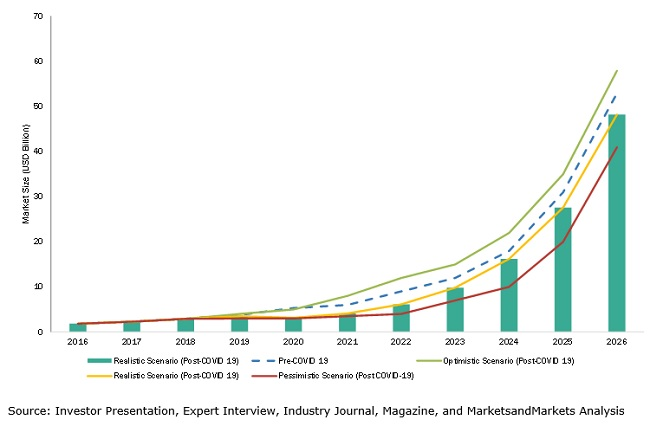
\includegraphics[width=1.0\linewidth]{img/digital-twin-market12.jpg}
    \caption[Übersicht Marktgröße \ac{DT}]{Marktentwicklung und Marktvorhersage für den Markt digitlaer Zwillinge \\Quelle: \citeauthor{markets2020} \citeurl{markets2020}} 
\end{figure}


Die Industrie ist allerdings nicht der einzige Ort, an dem \ac{DT}s vorteilhaft eingesetzt werden und wurden. Der Bereich der \ac{PHM} profitiert auch von der Nutzung digitaler Zwillinge. \citeauthor{tuegel2011reengineering} beschrieb bereits im Jahr \citeyear{tuegel2011reengineering} den Einsatz von \ac{DT}s zur Vorhersage des Lebenszyklus von Luftfahrzeugen. Dabei konnte durch die Abbildung in einer virtuellen Umgebung komplexe zusammenhängende Physiksimulationen durchgeführt werden. Damit konnten Vereinfachungen in verscheidenen Bereichen der Wartung eines Luftfahrzeugs erreicht werden.\autocites{tao2018digital}{tuegel2011reengineering} \\
Des weiteren lassen sich Forschungen für Anwendung im medizinischen Bereich finden. \autocites{barricelli2019survey}{tao2018digital}

\pagebreak

Große weltweit agierende Unternehmen, erkennen und fördern den gewonnenen Nutzen durch \ac{DT}s. Dazu zählen Unternehmen wie:
\begin{itemize}
    \item \textbf{Siemens:}\\ Siemens nutzt digitale Zwillinge im Bereich von Strom- und Abwasseranlagen in Finnland. Dort dienen die \ac{DT}s dazu, interne Abläufe zu optimieren und zu automatisieren.\autocite{tao2018digital}
    \item \textbf{Airbus:}\\ Airbus erreicht mithilfe von \ac{DT}s einen sehr hohen Automatisierungsgrad innerhalb der eigenen Fabriken. Konkret werden dort digitale Zwillinge eingesetzt, um Produktionslinien abzubilden, um so den Fertigungsgrad zu überwachen und Prozesse zu optimieren \autocite{tao2018digital}
    \item \textbf{Bosch:}\\ Bosch ist vor allem im Bereich der Softwareentwicklung für digitale Zwillinge tätig und bietet eine eigene Cloudlösung zur Verwaltung von \ac{DT}s an. Außerdem stellen sie viele Entwickler für verscheidene Eclipse Projekte bereit. \autocite{tao2018digital}
    \item \textbf{SAP SE:}\\ Die SAP SE kann durch digitale Zwillinge das \ac{PHM} von Unterwasseranlagen überwachen und Fernwartungen/-diagnosen durchführen. Somit entsteht eine immense Kostenersparnis, da Wartungseinsätze unter Wasser teuer sind. \autocite{tao2018digital}
\end{itemize}



\chapter{Problemstellung und Lösungsansatz}

Im folgenden Kapitel soll das Problem, welches bei der automatischen Erzeugung digitaler Zwillinge besteht, beschrieben werden. Dafür wird zuerst ein Ablauf dargestellt anhand dessen ein \ac{DT} erstellt wird. Dabei wird dann auf den aktuellen Ist-Zustand eingegangen. Es wird außerdem ein Soll-Zustand definiert, welcher erreicht werden soll, sodass spätere Konzepte daran gemessen werden können. Am Ende dieses Kapitels wird evaluiert, wo die Diskrepanz zwischen dem aktuellen Ist-Zustand und dem Soll-Zustand liegt.

\section{Die automatische Erzeugung digitaler Zwillinge}

Das automatische Erzeugen digitaler Zwillinge stellt nur ein Teilziel in einem größeren Prozess dar, dessen Ziel es ist, mittels eines digitalen Zwilling eine dauerhaft ansprechbare Schnittstelle zu einen Endgerät zu haben. Bei dem Teilprozess der Erzeugung digitaler Zwillinge spielen zwei Komponenten eine wesentliche Rolle. In Abbildung \vref{fig:high_level} sind die Kernkomponenten sowie deren Zusammenhang aufgezeigt. Im speziellen spielen dabei die Device Registry und der Digital Twin Provider eine Rolle.

Da es sich bei diesen beiden Bestandteilen um voneinander unabhänige Anwendungen handelt, muss eine dauerhafte Verbindung sichergestellt werden. Außerdem müssen Geräte, die innerhalb der Device Registry liegen auch über den Digital Twin Provider bereitgestellt werden können. Für beide Komponenten gibt es spezifische Heruasforderungen, welche im Folgenden näher betrachtet werden sollen.

\subsection{Device Registry}

Kernaufgabe der Device Registry ist es, wie in \vref{def:device_registry} noch einmal genauer beleuchtet, alle relevanten Endgeräte verwalten zu können. Um dieses Ziel erreichen zu können muss sichergestellt werden, dass die Vielzahl der im \ac{IoT} üblichen Kommunikationsprotokolle unterstützt wird. Würden nicht alle wichtigen Protokolle unterstützt werden, so wäre die Einsatzfähigkeit der Anwendung in Frage zu stellen. 

\pagebreak
Zu den wichtigsten Protokollen gehören unter anderem:
\begin{itemize}
    \item MQTT
    \item AMQP
    \item OPC-UA
    \item \ac{HTTP}/WS, etc.
\end{itemize}

\begin{figure}
    \centering
    \begin{tikzpicture}[node distance=4cm]
        \node (device) [io] {Endgerät};
        \node (dr) [process, right of=device, xshift=6cm] {Device Registry};
        \node (dts) [process, below of=dr] {Digital Twin Provider};
        \node (app) [startstop, below of=device] {Business Application};

        \draw [arrow] (device) -- node[anchor=south, align=left, text width=4cm] {sends telemetry data and authenticates} (dr);
        \draw [arrow] (dr) -- node[anchor=west, align=left, text width=2.5cm]{establishes connection and forwards telemetry data} (dts);
        \draw [arrow] (app) -- node[anchor=south, align=left, text width=4cm]{consumes information about digital twins} (dts);
        \draw [thick, dashed] (app) -- (device);
    \end{tikzpicture}
    \caption{Grobübersicht über die vorgeschlagene Architektur und deren Zusammenspiel\\ Quelle: Eigene Darstellung}
    \label{fig:high_level}
\end{figure}

Des weiteren gilt es die Herausforderung der Authentifizierung eines Endgerätes über die Device Registry zu lösen. Vor allem das Problem der Zugangsdaten muss gelöst werden, sodass ein problemloser Einsatz und Austausch von Endgeräten möglich ist, ohne administrativen Aufwand betreiben zu müssen. Dies hat auch Konsequenzen auf die wirtschaftlichen Auswirkungen, da ein geringer Wartungsaufwand auch geringere Kosten mit sich bringt. Ziel der in der Architektur verwendeten Device Registry sollte es dementsprechend sein, eine einfache, wartungsarme Authentifizierungsmethode bereitzustellen.

Außerdem muss eine Device Registry generisch einsetzbar sein. Eine Lösung, welche nur Geräte eines Anwenders unterstützt und keine Möglichkeit bereitstellt, eine Sichtbarkeitseinstellung oder Authentisierung gewisser Geräte für bestimmte Anwender vorzunehmen, würde den Einsatz einschränken. Auch hier würde eine Realisierung von mehr Anwendungsfällen zu höheren Kosten führen, da eventuell mehrere Serverressourcen bereitgestellt werden müssen.

\subsection*{Anforderungen an eine Device Registry}

Anhand obiger Analyse lassen sich mehrere Anforderungen an eine Device Registry ableiten:

\begin{enumerate}
    \item Bereitstellung einer einfachen Authentifizierungsmethode zwischen Endgerät und Device Registry
    \item Unterstützung möglichst vieler Kommunikationsprotokoll mit einer Möglichkeit zur Erweiterung um zusätzliche Protokolle
    \item Möglichkeit eines Einsatzes für mehrere Anwender innerhalb einer Device Registry. Eine Sichtbarkeitseinstellung muss möglich sein.
    \item Verarbeitung und Bereitstellung der Telemetriedaten der Endgeräte.
\end{enumerate}

Die Einführung einer Device Registry mit obigen Kriterien führt auch dazu, die Modularität zu erhöhen, da keine Funktionalität einer speziellen Device Registry vorausgesetzt wird. So kann auch im Falle eines Austauschs der Device Registry oder der Einführung einer Eigenentwicklung ohne Probleme migriert werden, sofern alle Kriterien erfüllt sind. Diese Modularität gilt es in allen Bereichen der Architektur zu erreichen.

\subsection{Digital Twin Provider}
\label{sec:dtp}

Die zweite wichtige Komponente im Teilprozess der automatischen Erstellung digitaler Zwillinge stellt der \textbf{Digital Twin Provider} dar. Seine Rolle im Gesamtprozess wird noch einmal in Abbildung \vref{fig:high_level} aufgezeigt.

Die Kernaufgabe eines \ac{DT} Providers stellt das zur Verfügungstellen der \textit{eigentlichen} digitalen Zwillinge dar. Das bedeutet ihm fällt die Verwaltung der Verbindung zwischen der in der Device Registry vorhandenen Geräte und dem \ac{DT} zu. Er muss sicherstellen, dass jeder digitaler Zwilling immer ansprechbar ist und verwertbare Informationen liefert. Zusätzlich fällt ihm die Aufgabe zu, sicherzustellen, dass \ac{DT}s eine Struktur haben, sodass eine Anfrage konsitente Ergebnisse liefert.

Zusätzlich ist es wichtig sogenannte \textit{virtuelle Eigenschaften} auf Basis vorhandener Daten erstellen zu können. Diese Eigenschaften können mithilfe von Funktionen berechnet werden. Daraus folgt eine Anforderung an den Digital Twin Provider: Dieser muss die Möglichkeit bereitstellen, Funktionen innerhalb einer abgesicherten Umgebung zur Berechnung anlegen zu können.

Gleichzeitig gilt eine Anforderung, welche bereits für die Device Registry von Relevanz war. Es muss die Möglichkeit geben, den \ac{DT} Provider durch mehr als einen Anwender nutzen zu können. Dafür müssen Mechanismen bereitgestellt werden, welche im Idealfall mit denen der Device Registry übereinstimmen.

Der Digital Twin Provider muss außerdem ein umfangreiches \enquote{Policy} Modul integrieren, um Zugriffsregeln bis auf Eigenschaftenebene eines \ac{DT}s bestimmen zu können. Dies ist von immenser Bedeutung, um ein durchgängiges Authentifizierungs- und Authorisierungskonzept aufrechtezuerhalten und externe Business Applications nach dem \enquote{least visibility} Prinzip bedienen zu können, auch um schädliche Zugriffe zu vermeiden.

Business Applikationen verwenden unterschiedlichste Kommunikationsprotokolle, um Daten zu erhalten. Um sicherzustellen, dass auch hier eine Vielzahl von Applikationen bedient werden kann, müssen, wie in der Device Registry, möglichst viele Protokolle unterstützt werden und nach Möglichkeit erweiterbar sein. Die bedeutensten Formate für Business Applikationen sind:

\begin{itemize}
    \item \texttt{HTTP/1.x} und \texttt{HTTP/2.0}\footnotetext{HTTP 2 ermöglicht neben dem parallelen Übertragen von Daten auch das Streamen von Datenpaketen. HTTP 1 dagegen setzt nur ein klassisches Request-Response Pattern um.\autocite{wijnants2018http}}
    \item Websockets
\end{itemize}

Diese Protokolle ermöglichen den einfachen Transfer von Telemetriedaten, sowohl auf Anfrage mittels \texttt{HTTP/1.x} oder auch kontinuierlich via Websockets oder \texttt{HTTP/2.0}.

Wichtig ist ebenfalls, das erzwingen einer konsistenten Struktur der digitalen Zwillinge. Dabei gilt es sicherzustellen, dass sowohl eine Struktur für die statischen Informationen (z.B. Modellnummer, Seriennummer, Standort, etc.) als auch die dynamischen Informationen (z.B. physische und virtuelle Sensoren) vorhanden ist. Dabei stellt es \textbf{nicht} die Aufgabe des \ac{DT} Providers dar, eine Verwaltungsstrutkur bereitzustellen, sondern nur auf Basis gegebener Strukturinformationen Validierungen durchzuführen und die Struktur zu erzwingen.

\subsection{Problemstellung}

Nun da die für das Problem relevanten Komponenten einmal näher beleuchtet, sowie deren grundlegenden Fähigkeiten beschrieben wurden, kann näher auf die Problematik eingegangen werden, zu welcher diese Arbeit eine Lösung bereitstellen soll. 

\pagebreak

Die Device Registry stellt ein umfangreiches Verwaltungssystem für die physischen Geräte bereit und ist mit Schnittstellen ausgestattet, welche von anderen Applikationen genutzt werden können. Eine dieser Applikationen ist der Digital Twin Provider, der Informationen zu Geräten aus der Registry nutzen kann, um digitale Zwillinge zu konstruieren und bereitzustellen. Ebenfalls können die \ac{DT}s an dieser Stelle verwaltet werden. Allerdings können digitale Zwillinge auch aufgrund der Anforderung einer festen Struktur \textbf{nicht} automatisch mit dem Senden der ersten Telemetriedaten erstellt werden. Zusätzlich dazu stellt die Anforderung der genauen Definition einer Policy ein Problem bei der automatischen Erzeugung dar.

Dies führt zu folgendem akkumulierten Problem.

\begin{problem}[Automatische Erzeugung digitaler Zwillinge]
    Durch die Modularität der Gesamtarchitektur sind die Device Registry und der Digital Twin Provider zwei voneinander getrennt operierende Systeme. Jedes dieser Systeme nutzt eigene Persitenzmechanismen, da unterschiedliche Anforderungen an die jeweiligen Systeme bestehen. Deshalb gibt es keinen geteilten Speicher, der einen integrierten automatischen Austausch der benötigten Informationen ermöglicht. Gleichzeitig fehlt eine Instanz, die digitalen Zwillingen Strukturinformationen bereitstellen kann. Die Integration dieser drei Komponenten muss automatisiert werden. Es wird ein System benötigt, welches die folgenden Kriterien erfüllt:

    \begin{itemize}
        \item Erkennen eines neu registrierten Gerätes innerhalb der Device Registry.
        \item Aufbauen einer stabilen Verbindung zum Transfer der Telemetriedaten zwschen Device Registry und Digital Twin Provider.
        \item Erstellen eines digitalen Zwillings mit Policy- und Strukturinformationen.
    \end{itemize}
\end{problem}

Der im Folgenden beschriebene Lösungsansatz versucht eine solche Applikation bereitzustellen und zeigt sowohl die Vor- als auch die Nachteile dieser Lösung auf.

\section{Lösungsansatz}

Es wird ein dritte Komponente hinzugefügt, welche die oben beschriebenen Aufgaben übernimmt. Dabei handelt es sich um einen autarken Service, welcher separat von den anderen Komponenten bereitgestellt werden kann. Diese Komponente lässt sich foglendermaßen in die Gesamtarchitektur integrieren:

\begin{figure}[h]
    \centering
    \begin{tikzpicture}[node distance=4cm and 4cm]
        \node (device) [io] {Endgerät};
        \node (dr) [process, right of=device, xshift=2cm] {Device Registry};
        \node (dts) [process, below of=dr] {Digital Twin Provider};
        \node (connector) [process, fill=green!30, right of=dr, yshift=-1.75cm] {Connector};
        \node (app) [startstop, below of=device] {Business Application};
    
        \draw [arrow] (device) -- (dr);
        \draw [arrow] (dr) -- (dts);
        \draw [arrow] (app) -- (dts);

        \draw [thick, dashed, color=red] (connector) -- (dr);
        \draw [thick, dashed, color=red] (connector) -- (dts);
        \draw [dashed] (connector) -| (device);
    \end{tikzpicture}
    \caption{Übersicht über die Integration des Connectors in die Gesamtarchitektur\\Quelle: Eigene Darstellung}
    \label{fig:high_level_conn}
\end{figure}

\pagebreak

In der Abbildung \vref{fig:high_level_conn} ist die Integration des Connectors in der Architektur beschrieben. Es lässt sich erkennen, dass dieser \textbf{keine hohe Kopplung} in seiner Integration mit sich bringt. Entsprechend kann dieser Service ohne Probleme zusätzlich über einen Server bereitgestellt werden. Es lässt sich auch erkennen, dass unter Umständen eine direkte Verbindung zum Endgerät für einen kurzen Zeitraum benötigt wird. Diese ist allerdings als Optional anzusehen, da sie nur in spezifischen Anwendungsszenarien von Bedeutung ist.

Diese Komponente benötigt zum operieren, wie in der Abbildung beschrieben, Zugriffe auf die Device Registry und den Digital Twin Provider. Die Aufgabe, die mithilfe des Connectors erledigt wird, besteht darin, im Falle eines neu registrierten Gerätes einen korrespondierenden \ac{DT} zu erstellen und diesen mit äquivalenter Sichtbarkeit auszustatten. Zusätzlich können Standardpolicies vergeben werden, die mitunter auch entsprechend der Sichtbarkeit individuell angepasst werden können. Ebenfalls fällt dem Connector die Aufgabe zu, benötigte Strukturinformationen während des Erstellens bereitzustellen. Dieser Vorgang kann sich von Anwendung zu Anwendung unterscheiden und lässt deshalb die genaue Umsetzung offen.\\
Es kann eine statische Vorlage hinterlegt werden, anhand welcher dann entsprechende Kriterien angewendet werden, oder es kann eine externe Registry genutzt werden, welche referenziert werden kann.

Optional wird auch eine Möglichkeit angeboten Metriken zur Verarbeitung in einer Prometheus-Instanz bereitzustellen. Diese bieten sowohl Einsicht in Hardwaremetriken, als auch konfigurierbare, softwarezentrierte Metriken. Die Hardwaremetriken sind mit einer flexiblen Implementierung ausgestattet, sodass es nicht von Bedeutung ist, ob der Service innerhalb einer Virtualisierungssoftware läuft oder direkt auf einem Server gestartet wird. Damit können mehr Anwendungsfälle realisiert werden.

\begin{figure}
    \centering
    \begin{tikzpicture}[node distance=3cm]
        \draw (-2.5,1) -- node[anchor=east, text width=2.75cm] {External Applications} (-2.5, -4);
        \node (dts) [process] {DT Provider Service};
        \node (drs) [process, right of=dts, xshift=4cm] {Device Registry Service};
        \node (ms) [process, below of=dts] {Monitoring Service};
        \node (cpa) [process, below of=drs] {Custom Protocol Adapters};
    
        \draw [dashed] (dts) -- (drs);
        \draw [dashed] (dts) -- (ms);
        \draw [dashed] (dts) -- (cpa);
        \draw [dashed] (drs) -- (cpa);
        \draw [dashed] (drs) -- (ms);
        \draw [dashed] (cpa) -- (ms);
    \end{tikzpicture}
    \caption{Interne Architektur des Connectors\\Quelle: Eigene Darstellung}
    \label{fig:internal_arch}
\end{figure}
Ebenfalls wird die interne Struktur des Connectors modular aufgebaut, sodass eine Erweiterung oder Einschränkung der Funktionalität einfach realisierbar ist. In Abbildung \vref{fig:internal_arch} ist ein exemplarischer Aufbau skizziert.

In der Abbildung wird deutlich, dass es sich bei den bereitgestellten Services um austauschbare und anpassbare Elemente handelt. Bei der konkreten Implementierung können die jeweiligen Services und Adapter entsprechend der konkreten gewählten Vertreter der einzelnen Komponenten (Device Registry, Digital Twin Provider, etc.) gewählt werden.


\chapter{Konzeptentwicklung}

Ziel des Konzeptes ist es eine möglichst automatisierte Erstellung digitaler Zwillinge ohne manuelle Interaktion bereitzustellen. Dies bringt verschiedene Vorteile mit sich, vor allem aber, können so dynamisch neue Zwillinge für neue Geräte generiert werden. Dabei ist es auch die Aufgabe bereits bestehende Geräte, im Falle einer Netzwerkpartition wieder mit ihrem entsprechenden Zwilling zu verbinden.\\
Dabei muss berücksichtigt werden, dass verschiedene Services bei dem Erstellen und dem Aufrechterhalten der Verbindung genutzt werden.

Eine wichtige Komponente stellt dabei die \textbf{Device Registry} dar. IBM definiert die Funktion einer Device Registry folgendermaßen:

\begin{definition}[Device Registry]
    \enquote{The Device Registry is the most important part of any IoT solution. With the registry, you can manage your device types and manage, maintain, and monitor the devices that you register.}\autocite{ibm_dr}
\end{definition}

Aus dieser Definition lassen sich mehrere wichtige Eigenschaften entnehmen. Zum einen stellt eine Device Registry einen zentralen Bestandteil dar. Dort liegt die Verwaltung der verscheidenen Geräte, welche alle entweder eigenständig oder miteinander kombiniert zur Erstellung digitaler Zwillinge genutzt werden können. Es geht auch hervor, dass die Art des Gerätes keine Rolle spielt - es können sogar verschiedene Typen verwaltet werden. Gleichzeitig dient es auch als zentrale Anlaufstelle, um die Authentizität von Geräten zu verifizieren. So muss eine Device Registry auch Mechanismen implementierne, der es ermöglicht tausende Geräte zu identifiezieren und zu verwalten.

Alle Bestandteile einer Device-Regisry lassen sich Abbildung \vref{fig:device_registry} erkennen. Von dieser Abbildung lässt sich auch eine exemplarischer Aufbau entnehmen, welche anderen Komponenten eine wichtige Rolle bei der Umsetzung einer Device Registry spielen. Für jeden Anwendungsfall eine eigene Device Registry aufzusetzen, Ressourcen für den Betrieb zu allokieren und zu warten gestaltet sich als unpraktisch. 
Deswegen sind die Registry verschiedener Anbieter \footnotetext{Google IoT Core, IBM, Eclipse Hono} mit einem Namespace System ausgestattet, sodass mehrere Nutzer abgetrennt voneinander innerhalb derselben Registry verwendet werden können.

\begin{figure}
    \centering
    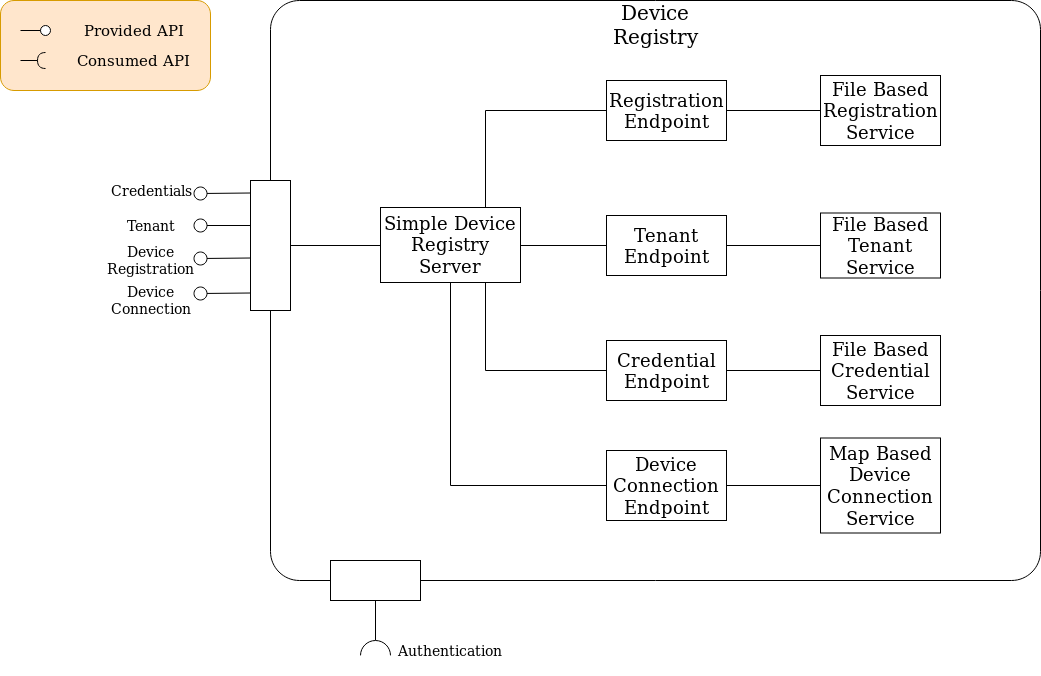
\includegraphics[width=0.75\linewidth]{img/device-registry.png}
    \caption[Bestandteile einer Device Registry]{Beispielhafter Aufbau einer Device Registry am Beispiel von Eclipse Hono. Quelle: \url{https://www.eclipse.org/hono/docs/architecture/component-view/device-registry.png}}
    \label{fig:device_registry}
\end{figure}

Inhärent bedeutet das, dass das Authentifizierungs- und Authorisierungssystem dieses Scoping unterstützen muss. Somit benötigt die Umsetzung der Authentifizierung eine genauere Begutachtung.

\section{Authentifizierung und Authorisierung von IoT Geräten}

Die Authentifizeriung von Geräten im IoT Bereich stellt eine Herausforderung dar. So stellt es sich als sehr unpraktisch dar, für jedes Gerät eigene Zugangsdaten zu generieren und auf dem Gerät zu hinterlegen, damit es sich bei der Device Registry identifizieren kann. Auch stellt es ein Sicherheitsproblem dar, sollten sich Geräte eigenständig in der Device Registry registrieren können, ohne vorher Beweisen zu können, dass sie Zugriff auf einen bestimmten Namespace haben. \\
Es gilt also eine Alternative zu finden, welche es ermöglicht Geräte im großen Stil mit Zugangsdaten auszustatten, welche allerdings nicht Geräteindividuell angepasst werden müssen.\\
Um das manuelle Hinterlegen geräteindividueller Zugangsdaten zu vermeiden müssen Alternativen untersucht werden, welche eine Vorauthentifizierung ermöglichen. 

Eigentliches Ziel der Authentifizierung ist der Nachweis einer behaupteten Eigenschaft einer Entität. Bricht man das Problem der Geräteauthentifizierung auf diesen Sachverhalt herunter, lässt sich erkennen, dass viele Konzepte der Krypthographie ähnliche oder gleiche Probleme bearbeiten. Ziel innerhalb der Kryptogrpahie ist unter anderen der Aufbau eines sicheren Kommunikationskanals zwischen verschiedenen Parteien. Umformuliert lässt sich das Problem folgendermassen darstellen:

\begin{problem}[Authentifizierung]
    Partei $A$ behauptet gegenüber Partei $B$, vertrauenswürdig zu sein.
\end{problem}

Dank dieser Transformation können nun Lösungen und Hilfsmmittel aus der Krypthographie zur Bearbeitung des Authentifizierungsproblems herangezogen werden.

Grundsätzlich gilt es innerhalb der Kryptographie zwei Formen der Verschlüsselung zu unterscheiden:

\begin{enumerate}
    \item Die \textbf{symmetrische Verschlüsselung}, welche darauf beruht, dass zwei Schlüssel ausgetauscht werden, die im Anschluss genutzt werden können, um eine sichere Kommunikation aufrecht zu erhalten.
    \item  Die \textbf{asymmetrische Verschlüsselung}, die mithilfe eines öffentlichen und eines privaten Schlüssels eine sichere Kommunikation aufbaut und aufrecht erhält.
\end{enumerate}

Ein bekannter Nachteil symmetrischer Verschlüsselungsmethoden, ist der Schlüsselaustausch und das Sicherstellen einer sicheren Kommunikation zwischen einer wachsenden Anzahl an Teilnehmern. Somit wäre eine symmetrische Art der Verschlüsselung suboptimal für einen Anwendungsfall bei digitalen Zwillingen.

Alternativ bieten sich dann noch Möglichkeiten asymmetrischer Verschlüsselungsarten an. Ein Vorteil dieser Art ist es, dass ein Schlüssel austausch sehr einfach erreicht werden kann, da der Aufbau der Verbindung auf Basis eines öffentlichen Schlüssels basiert. Nachteil dieser Methode ist es allerdings, dass der Verbindungsaufbau und die Geschwindigkeit der Verschlüsselung sehr langsam ist. Im speziellen wenn größere Datenmengen verschlüsselt werden müssen sind symmetrische Verschlüsselungen deutlich schneller. Außerdem stellen symmetrische Chiffren ein höheres Sicherheitsniveau zur Verfügung.

\subsection{Pre-Authentication via Zertifikat}
\label{sec:certificate}

Um soviele Vorteile wie möglich bei gleichzeitig so wenig Nachteilen wie nötig zu erhalten, ist es am sinnvollsten beide Ansätze miteinander zu kombinieren. Diese Idee wird bereits in der Internetkommunikation verwendet. Dabei wird mithilfe eines asymmetrischen Schlüsselpaars ein sichere Kanal zur Kommunikation für einen symmetrischen Schlüsselaustausch und die anschließende Verschlüsselung aufgebaut. \\
Durch den Einsatz eines Zertifikates können die beschriebenen Vorteile erreicht werden.

\subsubsection*{Aufbau eines Zertifikates}

Durch \citeauthor{RFC3280} wurde ein Standard definiert, welcher zur Authentifizierung mit Zertifikaten genutzt werden soll. Dabei handelt es sich um den X.509 Standard. In \vref{fig:cert_structure} wird die grundlegende Struktur eines Zertifikates beschrieben. Die für den Anwendungsfall wichtigsten Informationen lassen sich dabei in der Struktur eines \texttt{TBSCertificate} finden. Dazu zählen die Informationen über den Herausgeber (Issuer) und den Zweck (Subject) des Zertifikats. \autocite{RFC3280}

\begin{definition}[Subject]
    Where it is non-empty, the subject field MUST contain an X.500 distinguished name (DN).  The DN MUST be unique for each subject entity certified by the one CA as defined by the issuer name field. \autocite[Kapitel~4.1.2.6]{RFC3280}
\end{definition}

\begin{verbatim}
Certificate  ::=  SEQUENCE  {
    tbsCertificate       TBSCertificate,
    signatureAlgorithm   AlgorithmIdentifier,
    signatureValue       BIT STRING  }
TBSCertificate  ::=  SEQUENCE  {
    version         [0]  EXPLICIT Version DEFAULT v1,
    serialNumber         CertificateSerialNumber,
    signature            AlgorithmIdentifier,
    issuer               Name,
    validity             Validity,
    subject              Name,
    subjectPublicKeyInfo SubjectPublicKeyInfo,
    issuerUniqueID  [1]  IMPLICIT UniqueIdentifier OPTIONAL,
                            -- If present, version MUST be v2 or v3
    subjectUniqueID [2]  IMPLICIT UniqueIdentifier OPTIONAL,
                            -- If present, version MUST be v2 or v3
    extensions      [3]  EXPLICIT Extensions OPTIONAL
                            -- If present, version MUST be v3
    }
Version  ::=  INTEGER  {  v1(0), v2(1), v3(2)  }
CertificateSerialNumber  ::=  INTEGER
Validity ::= SEQUENCE {
    notBefore      Time,
    notAfter       Time }
Time ::= CHOICE {
    utcTime        UTCTime,
    generalTime    GeneralizedTime }
UniqueIdentifier  ::=  BIT STRING
SubjectPublicKeyInfo  ::=  SEQUENCE  {
    algorithm            AlgorithmIdentifier,
    subjectPublicKey     BIT STRING  }
\end{verbatim}
\label{fig:cert_structure}
\begin{center}
    \small \fullcite{RFC3280}
\end{center}

Um massenhaft Geräte zu authentifizieren kann während der Erstellung eines Namespaces/Tenants innerhalb der Device Registry ein Zertifikat inklusive korrespondierendem \textit{private Key} hinterlegt werden, dess Zweck darin besteht, als Identifikator für Geäte zu dienen. Bei einem Verbindungsversuch kann dann seitens des Authentifizierungsservice überprüft werden, ob das mitgesendete Zertifikat für den angefragten Tenant gültig ist. Anschließend können dann über dieses \enquote{sicheren Kanal} gerätespezifische Zugangsdaten generiert oder ausgetauscht werden.

Mithilfe dieser Gerätezugangsdaten kann eine zukünftige Identifikation der Geräte durchgeführt werden.

\begin{figure}[h]
    \centering
    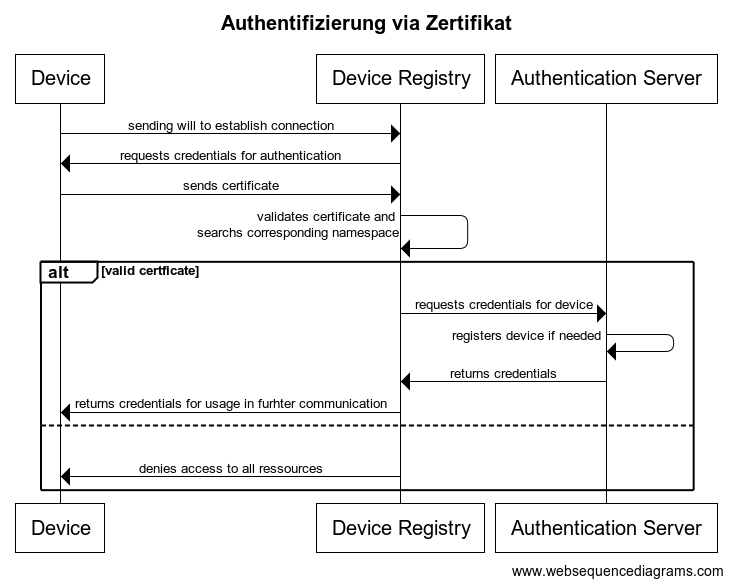
\includegraphics[width=1.0\linewidth]{img/device_authentication.png}
    \caption[Ablauf der Authentifizierung via Zertifikat]{Ablauf der Authentifizeriung eines Gerätes via Zertifikat.\\ Quelle: Eigene Darstellung}
    \label{fig:certificate}
\end{figure}

In Abbildung \vref{fig:certificate} ist zu erkennen, wie der Ablauf einer solchen Authentifizierung sein kann.

\subsection{Direkter Einsatz der Device Zugangsdaten}
\label{sec:credentials}

Werden die Zugangsdaten direkt auf dem Gerät hinterlegt, entsteht das oben beschriebene Problem. Das vorherige generieren dieser Zugansdaten bringt verschiedene Probleme mit sich, wenn die Geräte, die im späteren System eingesetzt werden, nicht final bekannt sind. Zudem muss außerdem noch da Problem gelöst werden, wie Zugangsdaten auf ein Gerät gelangen können.

Dieser Nachteil kann allerdins ignoriert werden, sollten es eigene Geräte sein, oder falls sich alle Geräte vor einem produktiven Einsatz in einer \enquote{Einrichtungsphase} befinden. Mithilfe dieser Methode könnte die Aufgabe der Zertifikaterstellung und -validierung von der Device Registry entfernt werden, was ein insgesamt klareres System erzeugt.

\subsection{Vergleich beider Authentifizierungsvarianten}

\begin{figure}
    \centering
    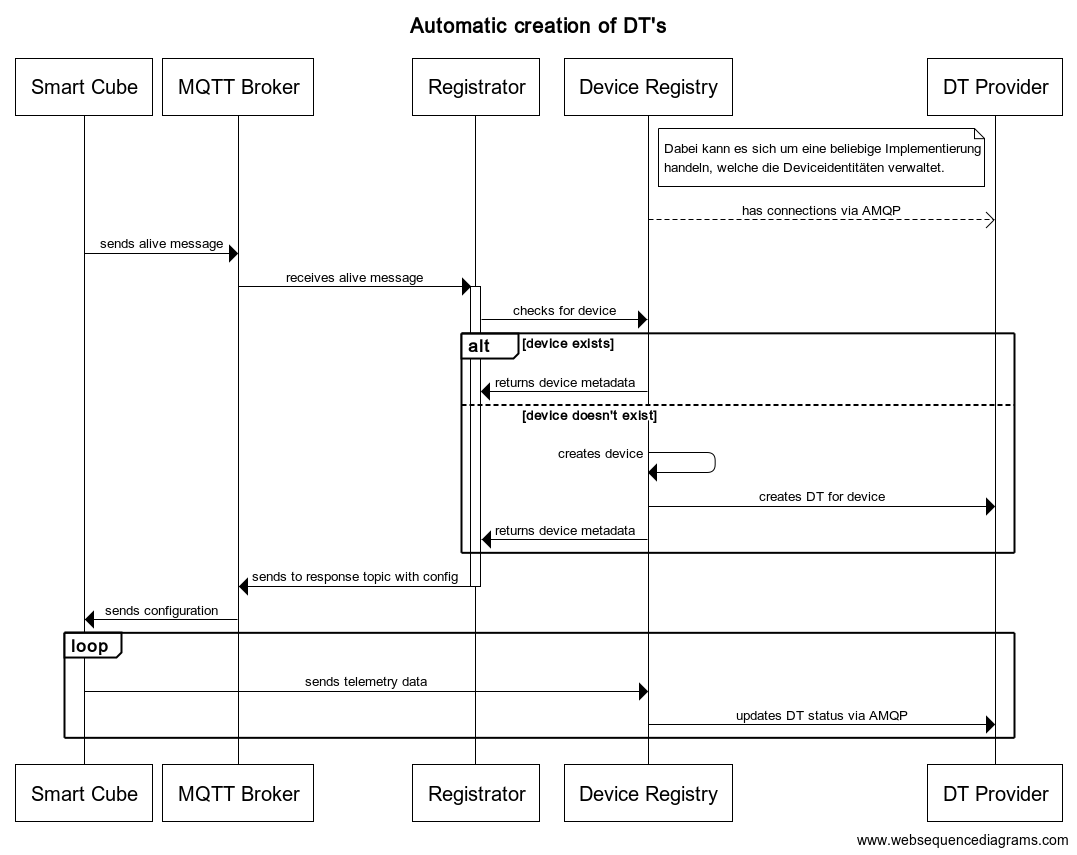
\includegraphics[width=1.0\linewidth]{img/automatic_creation.png}
    \caption[Automatische Erstellung digitaler Zwillinge]{Sequenzdiagramm des Ablaufs, sobald ein Gerät mit einem Netzwerk verbunden ist.\\Quelle: Eigene Darstellung.}
    \label{fig:automatic_creation}
\end{figure}

\begin{enumerate}
    \item Architekturkonzept
    \begin{itemize}
        \item Wieso Device-Registry? Anwendung, Anforderungen, Nutzen, etc.
        \begin{itemize}
            \item Eine Device Registry muss verschiedene Aufgaben erfüllen
            \item Muss Devices registrieren/verwalten können
            \item Verbindungen der Devices müssen abrufbar sein
            \item Authentifizierung/-sinformationen der Devices muss gespeichert werden
            \item bei generischer Nutzung $\rightarrow$ Scoping via namespace/tenant wichtig und muss dem device zugenordnet werden können
        \end{itemize}
        \item Authentifizierung, DaaS(Device as a Service), massenhafte Authentifizierung
        \begin{itemize}
            \item Was für verscheidene Methoden gibt es?
            \item Welche werden verwendet?
        \end{itemize}
        \item Common Schnittstellenformate, welche sind im Umlauf wie können sie zusammengeführt werden, sodass alle obigen Anforderungen noch laufen und erfüllt sind?
        \begin{itemize}
            \item Ein wenig die funktionalität und Idee hinter Eclipse Hono erklären. Dabei kurz die Grundlagen jedes Formats erklären
            \item MQTT
            \item AMQP
            \item HTTP
            \item WS (?)
        \end{itemize}
        \item Unterscheidung zwischen einer Device-Registry und der Speicherung als DT
        \begin{itemize}
            \item Hier liegt der Übergang der Arbeit; Es müssen von Geräten in der Device Registy DTs gebildet werden, nach möglichkeit automatisiert, sodass dann Daten des Gerätes übertragen werden
        \end{itemize}
        \item Was muss eine DT-Architektur mit sich bringen, damit Definition erfüllt Ist?
        \begin{itemize}
            \item Hier ein wenig auf die Ditto Idee eingehen.
            \item Konzept hinter Connections erklären; Was sind Connections, Was bringt das an Vorteilen mit sich
            \item Kombination zwischen Device-Registry und DT (hier liegt das Kernproblem!)
        \end{itemize}
        \item verschiedene Zugriffsarten auf die Daten eines DT
        \begin{itemize}
            \item Wie wird das alles exposed in Ditto?
            \item Kommt natürlich auf den Anwendungsfall an
            \item HTTP/WS
            \item AMQP
            \item usw.?
        \end{itemize}
        \item Welche Daten sind vorhanden und wie kann sichergestellt werden, dass ein speziell Modell für DT's vorliegt? $\rightarrow$ Hier kommt dan Vorto ins Spiel. Kurz das Konzept und Idee dahinter erläutern
        \begin{itemize}
            \item Vorto als Strukturregistry.
            \item Wieso ist das so wichtig
            \item welche vorteile gibt es, ein solches ding zu haben
        \end{itemize}
    \end{itemize}
    \item Softwarekonzept
    \begin{itemize}
        \item Müsste nochmal genau abklären, was damit gemeint ist
    \end{itemize}
\end{enumerate}

\chapter{Fazit und Ausblick}

In dieser Arbeit wurde ein Konzept vorgestellt, welches das automatische Erstellen digitaler Zwillinge ermöglicht. Dabei lag der Fokus vor allem darauf, das Zusammenspiel der einzelnen Komponenten zu untersuchen und Problemstellen zu identifizieren. Anschließend konnten aber auch Synergien festgestellt und genutzt werden. Gerade im Berech der Authentiizierung mussten einige Herausforderungen bewältigt werden. Unter anderem wurde dabei eine Methode vorgestellt, wie sich Geräte mithilfe eines Zertifikates ausweisen können, um anschließend mithilfe vor geräteindividuellen Zugansdaten operien zu können. Diese Methode unterstützt die dynamische Umgebung, und die sich ständig ändernde Anzahl an genutzten Geräten, ohne dass ein komplexer Registrierungsprozess nötig ist. Danach konnten die verschiedenen Komponenten zu einer Architektur zusammengeführt werden und mithilfe eines neuen Service erweitert werden, welcher die Aufgabe der Erstellung der digitalen Zwillinge übernimmt. 

Gerade im Bereich des zusätzlich entwickelten Services können im Rahmen weiterer Arbeiten einige Verbesserungen vorgenommen werden. In der aktuellen Implementierung wird nur eine bestimmte Kombination von Device Registry und Digital Twin Provider ohne die Verwendung einer Sturkturregistry ermöglicht. In einer Weiterentwicklung könnte die aktuelle Implementierung mit der Programmiersprache Golang zu Java portiert werden, sodass eine Integration in das Eclipse IoT Projekt möglich wäre. Diese Integration würde die Reichweite der Lösung erhöhen und dazu beitragen dem Ziel des Eclipse IoT Projektes einen industrieweiten Standard zu schaffen, näher zu kommen. Dazu müsste wie bereits erwähnt eine Migration des aktuellen Projektes vorgenommen werden und sichergestellt werden, dass weiterhin Eclipse Ditto\footnotetext{\url{https://www.eclipse.org/ditto/index.html}} als Digital Twin Provider unterstützt wird, aber zusätzlich auch Eclipse Hono\footnotetext{\url{https://www.eclipse.org/hono/}} als Device Registry und Eclipse Vorto\footnotetext{\url{https://www.eclipse.org/vorto/}} als Strukturregistry verwendet werden kann. 

Eine weitere Möglichkeit der Erweiterung liegt darin, weitere Methoden der Authentifizierung zu untersuchen. Es können unteranderem Ansätze von \citeauthor{fang2020fast} genutzt werden um mithilfe von Machine Learning Verbesserungen bei der Sicherheit großer IoT Anwendungsfälle zu erreichen. \autocite{fang2020fast} So könnte untersucht werden, ob und inwiefern das Konzept umsetzbar ist und welche Auswirkungen es konkret auf die Nutzung digitaler Zwillinge hätte. 

%	Literaturverzeichnis
\clearpage
\ihead{}
\printbibliography[title=Literaturverzeichnis]
\cleardoublepage

% Der Anhang beginnt hier - jedes Kapitel wird alphabetisch aufgezählt. (Anhang A, B usw.)
% \appendix
% \ihead{\appendixname~\thechapter} % Neue Header-Definition


\end{document}
